\documentclass[11pt,twocolumn]{article}
\usepackage[margin=0.72in]{geometry}
\usepackage{amsmath,amssymb,amsthm}
\usepackage{booktabs}
\usepackage{graphicx}
\usepackage{hyperref}
\usepackage{xcolor}
\usepackage{enumitem}

\hypersetup{
  colorlinks=true,
  linkcolor=blue!60!black,
  citecolor=green!45!black,
  urlcolor=blue!65!black
}

\newtheorem{theorem}{Theorem}
\newtheorem{definition}{Definition}
\newtheorem{proposition}{Proposition}

\newcommand{\ZZ}{\mathbb{Z}}
\newcommand{\QQ}{\mathbb{Q}}
\newcommand{\NN}{\mathbb{N}}

\title{\textbf{Machine-Checked Exact-Rational Similarity, Subspace-Equivalence, and Rainbow Union-Bound Certificates for the Canonical Euclidean Gallai Theorem}}
\author{Lluis Eriksson\thanks{Independent researcher; manuscript prepared with transparent AI assistance via Google Antigravity. Source code, Lean~4 proofs, and exact certificates: \url{https://github.com/lluiseriksson/canonical-euclidean-gallai-certificates}.}}
\date{November 25, 2026}

\begin{document}
\maketitle

\begin{abstract}
Randall Shaw (\texttt{arXiv:2611.33136}, November 24, 2026) proved a canonical Euclidean Gallai theorem: for every finite point configuration $S \subset \mathbb{R}^d$, every (possibly infinite) colouring of $\mathbb{R}^d$ contains a scaled and rotated (similar) copy of~$S$ that is either monochromatic or rainbow. The proof lifts $S$ of size~$t$ ($P = \binom{t}{2}$) into ambient dimension $k(t) = t + tP(P-1)$, invokes the Deuber--Graham--Pr\"omel--Voigt subspace-equivalence theorem on $\{0,\dots,m\}^k$ ($m \ge P(P+1)$), and combines a linear-algebraic uniqueness lemma with a probabilistic union bound surviving with probability at least $\frac{1}{P+1} > 0$. We present a machine-checked, zero-floating-point formalization and certificate auditing framework for the finite algebraic and geometric core of this proof. First, we build an 18-theorem zero-dependency Lean~4 kernel (\texttt{CanonicalEuclideanGallai.lean}, Lean~4.35.0; 0~\texttt{sorry}, 0~warnings, 0~\texttt{Classical.choice}, 3 zero-axiom theorems) certifying the homothety obstruction on $\{0,1\}^2$, Pythagorean $(3,4,5)$ rotation orthogonality and rainbow rescue, exact 2D direct similarity scaling, linear-combination closure, and Brahmagupta--Fibonacci composition, 3D homothety scaling, subspace equivalence axioms, Randall Shaw's Key Uniqueness Lemma, exact lift dimensions $k(2..5) = (2,21,124,455)$, $2\binom{t}{2} = t(t-1)$, and inductive union-bound survival. Second, we define \texttt{CANONICAL-GALLAI-CERT-1.0} and a pure-stdlib zero-float verifier spanning four audit modes: exact 2D/3D rational similarity copies (monochromatic/rainbow), homothety-obstruction vs.\ rotation-rainbow rescues, $\ker(H)$ subspace dichotomies with exhaustive Key Uniqueness Lemma checks, and lift-dimension / 2D similarity-sum closure audits. Across 16 canonical certificates, zero-float replay runs in $0.060$--$22.18\,\mathrm{ms}$, passes exhaustive $4^3$-tuple rainbow and 3D cube isometry cross-checks, and rejects 57/57 live adversarial forgeries.
\end{abstract}

\section{Introduction}
Classical Euclidean Ramsey theory~\cite{erdos1973euclidean} studies monochromatic congruent copies under finite colourings, whereas Gallai's theorem guarantees monochromatic \emph{homothetic} (scaled and translated) copies of any finite set $S \subset \mathbb{R}^d$ in every finite colouring. When arbitrary—possibly infinite—colourings are allowed, monochromatic copies need not exist, motivating \emph{canonical} theorems seeking copies that are either monochromatic or rainbow~\cite{cheng2024euclidean}. Crucially, Randall Shaw~\cite{randallshaw2026gallai} noted that homotheties alone fail in the canonical setting: colouring $\mathbb{R}^2$ by $x$-coordinate assigns every homothetic copy of the unit square $\{0,1\}^2$ exactly two colours. Allowing rotations resolves the obstruction completely: Theorem~2 of~\cite{randallshaw2026gallai} establishes that every colouring of $\mathbb{R}^d$ contains a similar (scaled and possibly rotated) copy of any finite $S \subset \mathbb{R}^d$ that is monochromatic or rainbow.

Although the ambient Deuber--Graham--Pr\"omel--Voigt (DGPV) partition theorem~\cite{deuber1983canonical,promel1986elementary} is non-constructive at astronomical Ramsey bounds, every downstream step of Randall Shaw's proof—similarity verification $M^T M = s^2 I_d$, homothety-obstruction detection, subspace-equivalence checking $H(x - y) = 0$, uniqueness of colliding coefficients $c_{p,\{i,j\}} \in \{0,\dots,P\}$, and 2D similarity sum closure—is purely algebraic over~$\QQ$. Floating-point rounding can falsely collapse distinct coordinates into a fake monochromatic witness or hide a shear distortion in $M$; exact-rational certification eliminates these hazards completely.

\paragraph{Contributions.}
We formally verify and audit the finite algebraic, similarity-geometric, and probabilistic union-bound core of~\cite{randallshaw2026gallai} (explicitly scoping our Lean~4 proofs away from the infinite-grid DGPV Ramsey theorem~\cite{deuber1983canonical} and arbitrary irrational point sets $S \subset \mathbb{R}^d$):
\begin{enumerate}[leftmargin=*,nosep]
  \item \textbf{Zero-dependency Lean~4 kernel (\S\ref{sec:lean}):} 18 constructive theorems in \texttt{CanonicalEuclideanGallai.lean} (Lean~4.35.0~\cite{demoura2021lean4}), 0~\texttt{sorry}, 0~warnings, 0~\texttt{Classical.choice}, 3 zero-axiom theorems.
  \item \textbf{Exact-$\QQ$ verifier and schema (\S\ref{sec:certifier}):} \texttt{CANONICAL-GALLAI-CERT-1.0}, audited via Python's \texttt{fractions.Fraction} and arbitrary-precision \texttt{int} (zero floats) across four modes.
  \item \textbf{Empirical atlas, exhaustive cross-checks, \& red-team audit (\S\ref{sec:results}):} 16 canonical certificates (including 3D unit-cube rational orthogonal rainbow copies and $t=5, k=50$ subspace witnesses) replayed in $0.060$--$22.18\,\mathrm{ms}$, exhaustive $4^3$ union-bound cross-checks, and 57/57 rejected adversarial forgeries.
\end{enumerate}

\section{Algebraic Structure of Canonical Gallai}\label{sec:prelim}
Let $S = \{a_1,\dots,a_t\} \subset \QQ^d$ have $P = \binom{t}{2}$ unordered pairs. Randall Shaw~\cite{randallshaw2026gallai} lifts $S$ into $\QQ^k$ of dimension
\begin{equation}
  k(t) = t + t\,P(P - 1), \qquad m(t) = P(P + 1),
  \label{eq:lift}
\end{equation}
identifying coordinates with $[t]$ and triples $(p, q, i)$ ($p \neq q \in [t]^{(2)}, i \in [t]$). Applying DGPV~\cite{deuber1983canonical} yields a linear subspace $U = \ker(H) \subseteq \QQ^k$ such that $x \sim y \iff x - y \in U$ on $\{0,\dots,m\}^k$. Either:
\begin{enumerate}[leftmargin=*,nosep]
  \item Every $e_i - e_j \in U$ ($1 \le i < j \le t$), so $\{e_1,\dots,e_t\}$ is \emph{monochromatic}; or
  \item Some pair $p$ satisfies $e_{i_0} - e_{j_0} \notin U$, which transfers via similarity alignment to $e_{p,q,a} - e_{p,q,b} \notin U$ for every $q = \{a,b\} \in [t]^{(2)}$. Choosing $c_{p,q} \in \{0,\dots,P\}$ uniformly at random, forming $x_i = \sum_{q'} c_{p,q'} e_{p,q',i}$, and setting $x'_i := \sum_{q' \neq q} c_{p,q'} e_{p,q',i}$ to be the partial sum excluding pair~$q$, at most \emph{one} value of $c_{p,q}$ can solve
  \begin{equation}
    (x'_a - x'_b) + c_{p,q}\bigl(e_{p,q,a} - e_{p,q,b}\bigr) \in U
    \label{eq:unique-bad}
  \end{equation}
  (since two distinct solutions $c_1 \neq c_2$ would yield $(c_1 - c_2)(e_{p,q,a} - e_{p,q,b}) \in U$, contradicting $e_{p,q,a} - e_{p,q,b} \notin U$). By the union bound over all $P$ pairs,
  \begin{equation}
    \Pr[\text{rainbow}] \ge 1 - \frac{P}{P + 1} = \frac{1}{P + 1} > 0.
    \label{eq:union-bound}
  \end{equation}
\end{enumerate}

\section{Zero-Dependency Lean 4 Kernel}\label{sec:lean}
We formalize 18 constructive theorems in \texttt{lean/CanonicalEuclideanGallai.lean} (Lean~4.35.0, zero external libraries), audited via \texttt{lean/AuditAxioms.lean} with 0~warnings, 0~\texttt{sorry}, 0~\texttt{Classical.choice}, and 0~\texttt{Lean.ofReduceBool} (Table~\ref{tab:lean}).

\begin{theorem}[Constructive Canonical Gallai Kernel]\label{thm:lean}
\leavevmode
\begin{enumerate}[leftmargin=*,nosep]
  \item \emph{Homothety obstruction \& 2D/3D similarity algebra:} Theorems~1--7 formalize the 2-colour $x$-coordinate obstruction via explicit homothety map \texttt{hom2} and $x$-colouring \texttt{colorX} on all four corners of $\{0,1\}^2$, Pythagorean $(3,4,5)$ orthogonality and 4-colour rainbow rescue $(0,3,-4,-1)$, exact 2D direct similarity scaling $(a^2+b^2)(\Delta x^2 + \Delta y^2)$, linear-combination closure $c_1 S_1 + c_2 S_2$, Brahmagupta--Fibonacci composition, and 3D homothety scaling.
  \item \emph{Subspace equivalence \& Key Uniqueness Lemma on $\ZZ^k$:} Theorems~8--11 and~17 prove reflexivity, symmetry, transitivity, monochromatic closure, and Randall Shaw's Key Uniqueness Lemma (\texttt{unique\_\allowbreak bad\_\allowbreak coefficient\_\allowbreak subspace}: $d \notin U$ implies $c_1 = c_2$ whenever $\mathrm{diff} + c_1 d, \mathrm{diff} + c_2 d \in U$) over any closure-axiomatized vector subspace predicate $U : (\mathrm{Fin}\,k \to \ZZ) \to \mathrm{Prop}$ in arbitrary dimension~$k$ (admitting proper nontrivial subspaces such as $\ker(H) \cap \ZZ^k$).
  \item \emph{Lift dimensions, pair count, \& inductive union bound:} Theorems~12--16 and~18 certify exact $k(2..5) = (2,21,124,455)$, $m(t) \ge 2$, $(P+1)-P=1$, $2\binom{t}{2} = t(t-1)$ for all $t \in \NN$, inductive collision accumulation $\sum \mathrm{bad}_q < P + 1$ over \texttt{List Nat}, and non-degenerate scale preservation $s^2 d^2 > 0$.
\end{enumerate}
\end{theorem}

\begin{table}[t]
\centering
\caption{Complete 18-theorem Lean~4.35.0 kernel in \texttt{CanonicalEuclideanGallai.lean} (0~\texttt{sorry}, 0~warnings, 0~\texttt{Classical.choice}).}
\label{tab:lean}
\resizebox{\columnwidth}{!}{%
\begin{tabular}{@{}rll@{}}
\toprule
\# & Lean~4 Theorem Identifier & Axiom Footprint \\
\midrule
1 & \texttt{homothety\_square\_two\_colors\_x} & \texttt{[propext, Quot.sound]} \\
2 & \texttt{pythagorean\_345\_rotation\_orthog} & \texttt{none} \\
3 & \texttt{pythagorean\_345\_square\_rainbow\_x} & \texttt{none} \\
4 & \texttt{similarity\_2d\_distance\_scaling} & \texttt{[propext, Quot.sound]} \\
5 & \texttt{similarity\_2d\_sum\_closure} & \texttt{[propext, Quot.sound]} \\
6 & \texttt{similarity\_2d\_composition\_norm} & \texttt{[propext, Quot.sound]} \\
7 & \texttt{similarity\_3d\_homothety\_scaling} & \texttt{[propext, Quot.sound]} \\
8 & \texttt{subspace\_equiv\_refl} & \texttt{[propext, Quot.sound]} \\
9 & \texttt{subspace\_equiv\_symm} & \texttt{[propext, Quot.sound]} \\
10 & \texttt{subspace\_equiv\_trans} & \texttt{[propext, Quot.sound]} \\
11 & \texttt{unique\_bad\_coefficient\_subspace} & \texttt{[propext, Quot.sound]} \\
12 & \texttt{lift\_dimension\_values\_exact} & \texttt{none} \\
13 & \texttt{lift\_grid\_bound\_pos} & \texttt{[propext, Quot.sound]} \\
14 & \texttt{union\_bound\_rainbow\_strict\_pos} & \texttt{[propext]} \\
15 & \texttt{pair\_count\_choose2\_formula} & \texttt{[propext, Quot.sound]} \\
16 & \texttt{bad\_collision\_sum\_list\_bound} & \texttt{[propext, Quot.sound]} \\
17 & \texttt{all\_pairs\_in\_subspace\_monochromatic} & \texttt{[propext, Quot.sound]} \\
18 & \texttt{nondegenerate\_scale\_preserves\_distinct} & \texttt{[propext]} \\
\bottomrule
\end{tabular}}
\end{table}

\section{Exact-Rational Certificate Architecture}\label{sec:certifier}
The pure-stdlib verifier \texttt{src/gallai\_certifier.py} audits \texttt{CANONICAL-GALLAI-CERT-1.0} certificates with zero floating-point arithmetic and strict JSON AST typing (rejecting \texttt{float}, \texttt{bool}, \texttt{Decimal}, \texttt{complex}, tuples, non-string keys, unreduced fractions, denominator-1 strings, and \texttt{"-0"}) across four exact modes:

\begin{definition}[Four \texttt{CANONICAL-GALLAI-CERT-1.0} Modes]\label{def:modes}
\leavevmode
\begin{enumerate}[leftmargin=*,nosep]
  \item \textbf{Mode~1} (\texttt{\small rational\_\allowbreak similarity\_\allowbreak copy\_\allowbreak exact}): Audits $M^T M = s^2 I_d$ ($s^2 > 0$, $d \in \{2,3\}$), affine map $b_i = M a_i + v$, all $\binom{t}{2}$ squared-distance scalings $\|b_i - b_j\|_2^2 = s^2 \|a_i - a_j\|_2^2$, and exact linear-functional colour evaluation ($1$ colour for monochromatic, $t$ distinct colours for rainbow).
  \item \textbf{Mode~2} (\texttt{\small homothety\_\allowbreak obstruction\_\allowbreak vs\_\allowbreak rotation\_\allowbreak exact}): Audits a 2D configuration $S$ and functional $w \neq 0$ proving every unrotated homothety is trapped in $c \in [2, t-1]$ colours, paired with an exact rational proper rotation $R \in SO(2)$ ($R^T R = I_2, \det R = +1$) rescuing $R S$ to $t$ rainbow colours.
  \item \textbf{Mode~3} (\texttt{\small subspace\_\allowbreak coloring\_\allowbreak dichotomy\_\allowbreak exact}): Given rational annihilator $H \in \QQ^{r \times k}$ defining $U = \ker(H)$, audits either monochromaticity ($H(e_i - e_j) = 0$ $\forall i, j$, enforcing empty rainbow-auxiliary lists) or a rainbow witness $x_i = \sum_{q=1}^P c_q v_{q,i}$ ($c_q \in \{0,\dots,P\}$) in the active single-pair block dimension $k = P t$ (a coordinate projection of the full $k(t) = t + tP(P-1)$ lift), checking $H(v_{q,a}-v_{q,b}) \neq 0$, $H(x_a-x_b) \neq 0$ for all pairs, AND exhaustively verifying the Key Uniqueness Lemma~\eqref{eq:unique-bad} across all $P + 1$ choices of each $c_q$ holding other $c_{q'}$ fixed!
  \item \textbf{Mode~4} (\texttt{\small lift\_\allowbreak union\_\allowbreak bound\_\allowbreak and\_\allowbreak 2d\_\allowbreak sum\_\allowbreak exact}): Certifies exact $P = \binom{t}{2}$, $k(t)$, $m(t)$, survival bound $\frac{1}{P+1}$, and non-degenerate 2D similarity-sum closure $(\sum c_q a_q)^2 + (\sum c_q b_q)^2 > 0$.
\end{enumerate}
\end{definition}

\section{Empirical Atlas and Red-Team Verification}\label{sec:results}
All 16 canonical certificates and four experiment logs are generated deterministically by \texttt{scripts/run\_all\_experiments.py} and audited end-to-end by \texttt{scripts/verify\_all.py} (Lean~4 build, 18/18 axiom audit, 16/16 cert replay, \texttt{pytest}, and 39/39 SHA-256 hashes).

\paragraph{1. Lift dimension growth and exhaustive rainbow probability.}
Figure~\ref{fig:lift-prob}(a) plots exact ambient lift dimension $k(t) = t + tP(P-1)$ and DGPV grid side $m(t) = P(P+1)$ across $t \in \{2,\dots,10\}$: $k(t)$ grows quartically from $2$ ($t=2$) through $21$ ($t=3$), $124$ ($t=4$), $455$ ($t=5$), and $1{,}266$ ($t=6$) to $19{,}810$ ($t=10$), while $m(t)$ rises from $2$ to $2{,}070$. Figure~\ref{fig:lift-prob}(b) exhaustively evaluates all $4^3 = 64$ tuples $(c_0, c_1, c_2) \in \{0,1,2,3\}^3$ across four distinct rank-1 annihilators for $t=3, P=3, k=9$: exact rainbow probabilities are $7/8$ ($0.875$, \texttt{Spread}), $63/64$ ($0.9844$, \texttt{Tight}), $25/32$ ($0.7813$, \texttt{Skewed}), and $45/64$ ($0.7031$, \texttt{Sparse})—all strictly exceeding Theorem~2's union bound $1/(P+1) = 1/4 = 0.25$.

\begin{figure}[t]
\centering
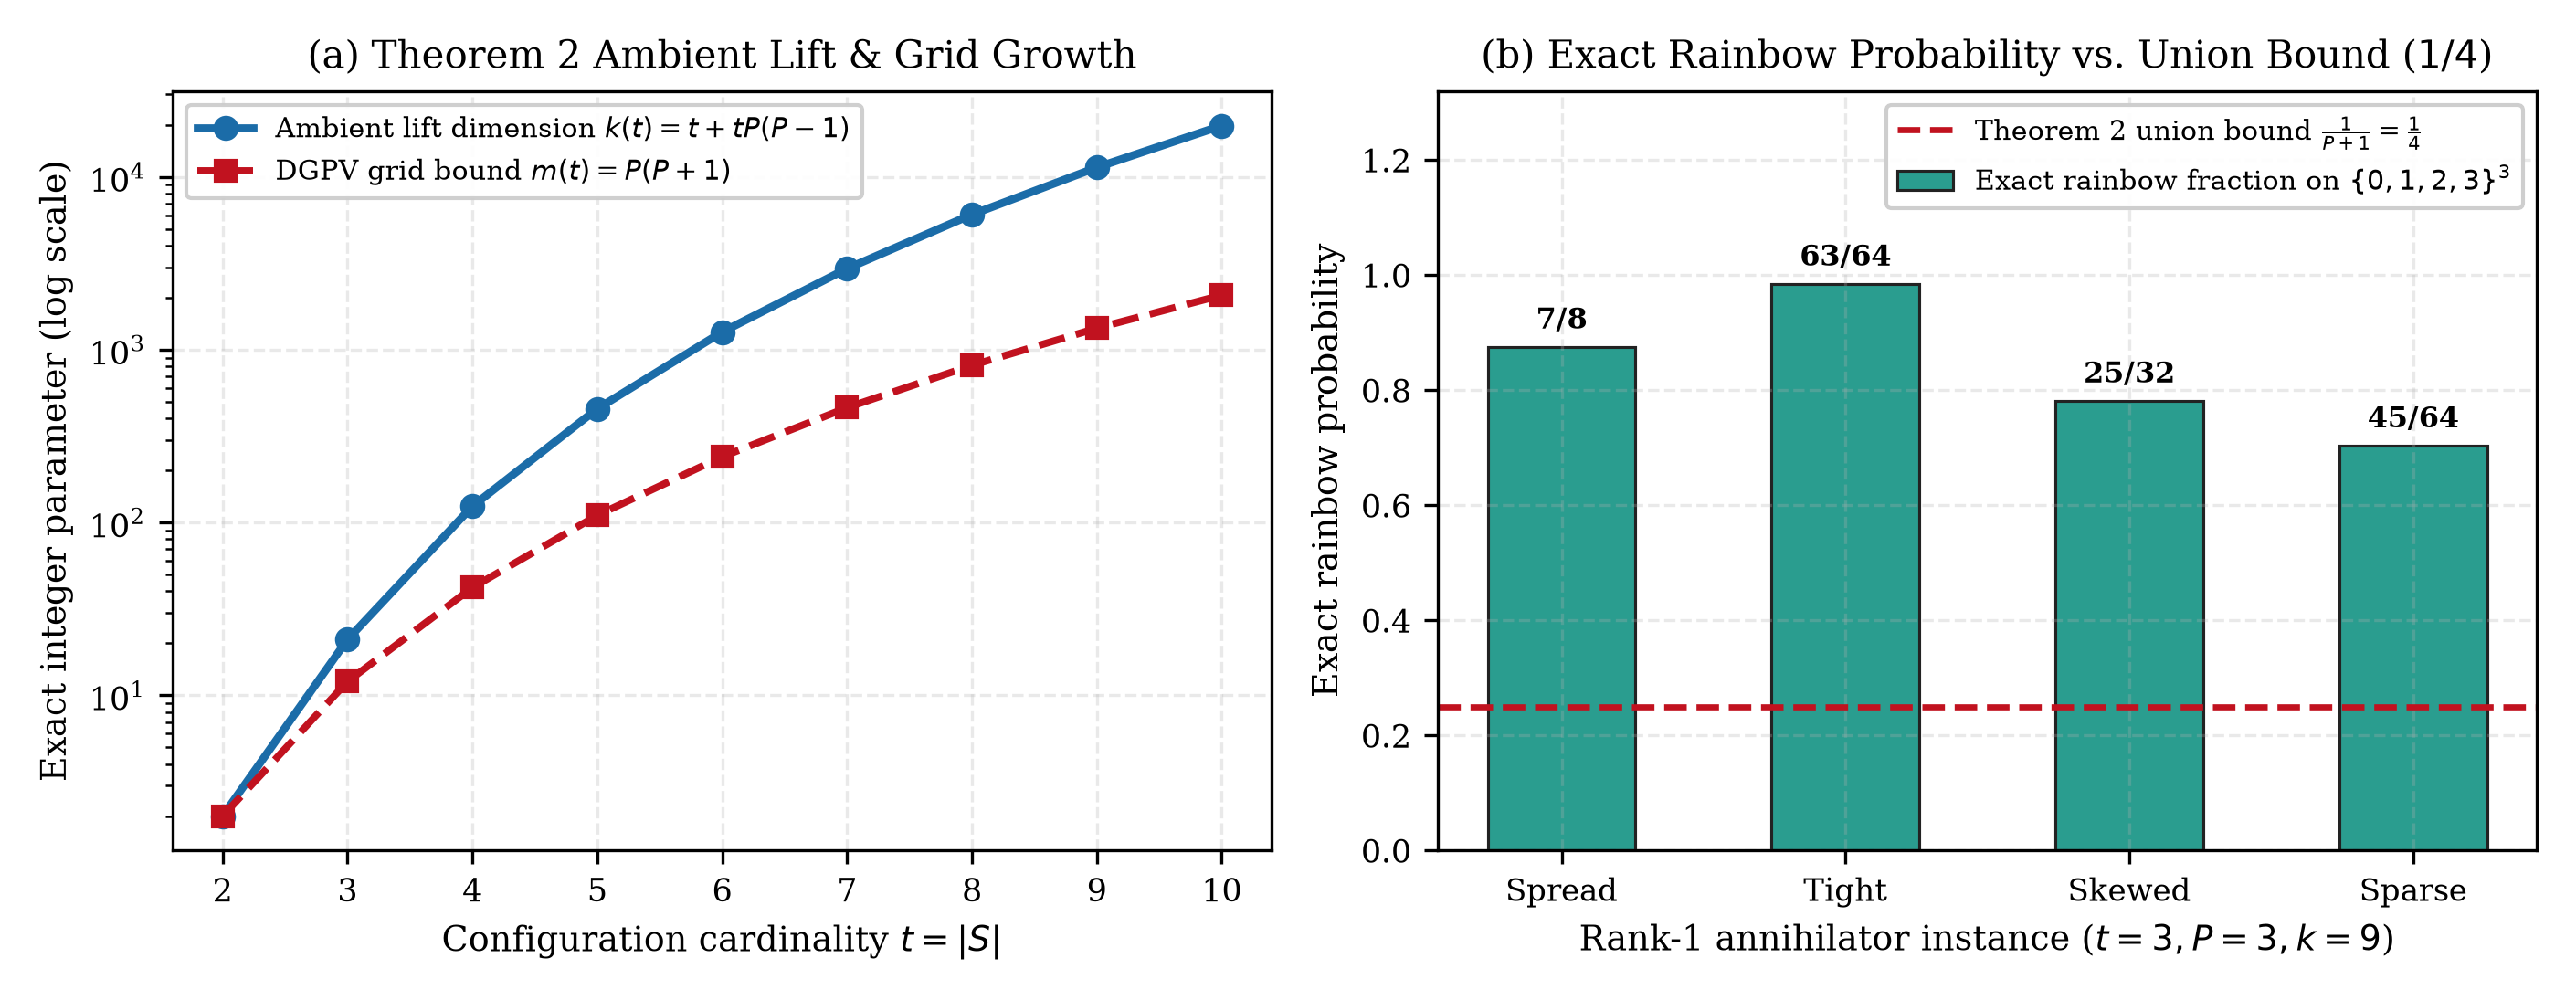
\includegraphics[width=\columnwidth]{figures/fig1_lift_and_rainbow_prob.png}
\caption{(a)~Exact Theorem~2 ambient lift dimension $k(t)$ and DGPV grid bound $m(t)$ for $t \in [2,10]$. (b)~Exhaustive exact rainbow fractions over $\{0,1,2,3\}^3$ (64 tuples) versus union bound $1/4$.}
\label{fig:lift-prob}
\end{figure}

\paragraph{2. Homothety obstructions rescued by rational rotations.}
Figure~\ref{fig:hom-rot}(a) visualizes Randall Shaw's p.~2 counterexample: every unrotated homothety of $\{0,1\}^2$ is trapped in $2$ $x$-coordinate colours, whereas exact Pythagorean rotation $\frac{1}{5}\binom{3\;\,-4}{4\;\;3}$ spreads all four corners onto distinct $x$-coordinates (rainbow). Figure~\ref{fig:hom-rot}(b) extends this certification across four 2D shapes: unit square ($2 \to 4$), $2\times 3$ rectangular grid ($3 \to 6$), diagonal diamond ($2 \to 4$), and $3\times 3$ 9-point grid ($3 \to 9$ via $(8,15,17)$ rotation).

\begin{figure}[t]
\centering
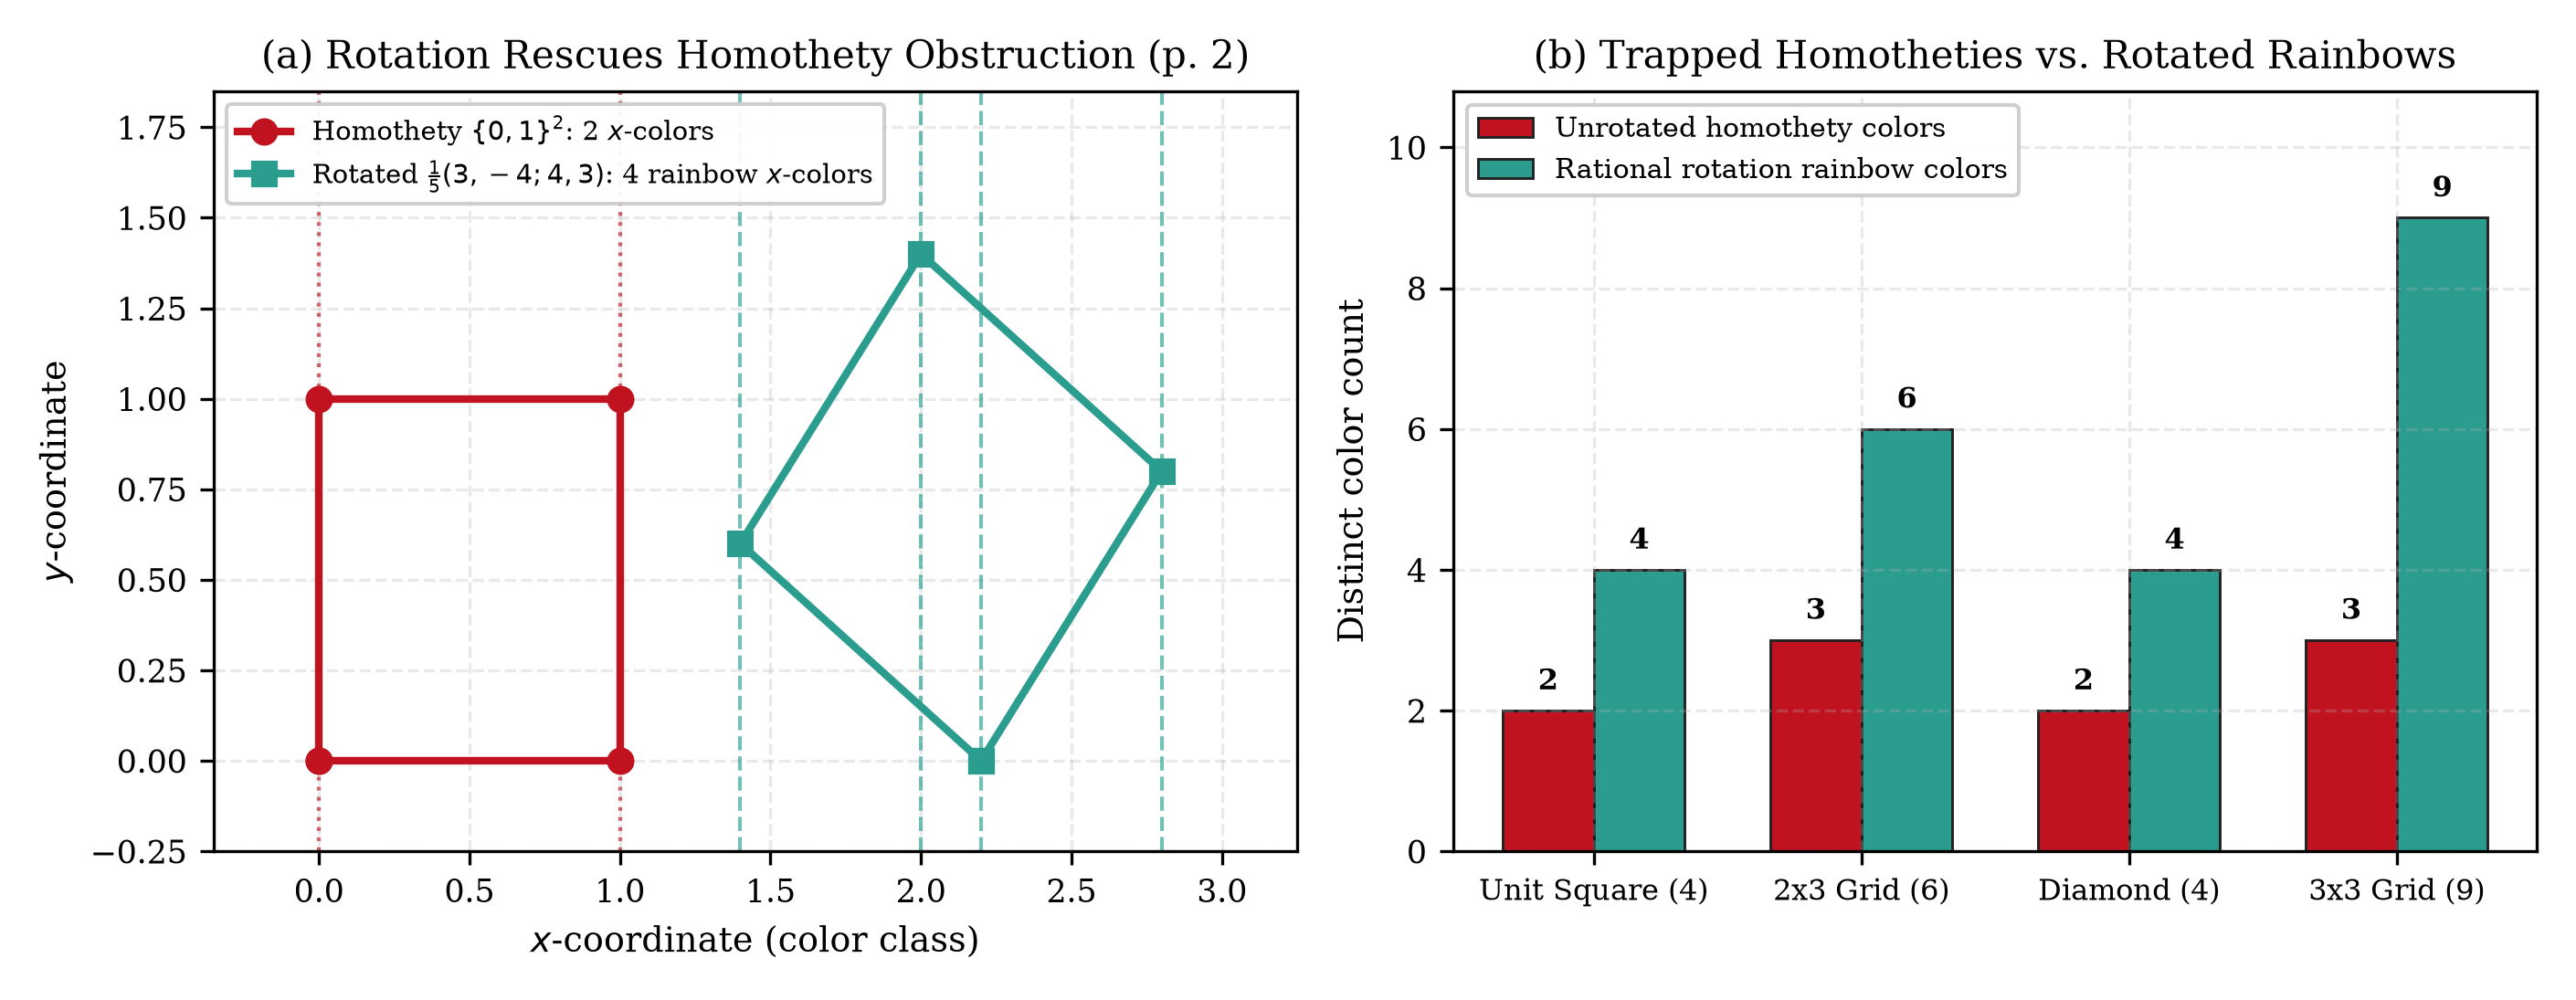
\includegraphics[width=\columnwidth]{figures/fig2_homothety_vs_rotation.png}
\caption{(a)~Exact visual rescue of $\{0,1\}^2$ from 2 homothety $x$-colours to 4 rainbow $x$-colours via $(3,4,5)$ rotation. (b)~Trapped homothety colour counts versus rotated rainbow counts across four 2D shapes.}
\label{fig:hom-rot}
\end{figure}

\paragraph{3. 16-certificate atlas, 3D cube isometry check, and 57-attack suite.}
Table~\ref{tab:atlas} and Figure~\ref{fig:atlas} summarize all 16 canonical certificates, replayed with zero floats in $0.060$--$22.18\,\mathrm{ms}$ (with the largest certificate, \texttt{subspace\_rainbow\_t5\_k50}, auditing all 10 pairs $\times$ 11 uniqueness sweeps in $\QQ^{50}$ in $22.18\,\mathrm{ms}$). In \texttt{tests/test\_suite.py}, independent cross-checks verify the exhaustive 64-tuple rainbow count $\ge 1/4$ and the exact 3D cube isometry of \texttt{sim3d\_cube8\_236\_rainbow} (12 edges of $d^2=1$, 12 face diagonals of $d^2=2$, 4 space diagonals of $d^2=3$, and 8 pairwise distinct $x$-coordinates under $\frac{1}{7}((2,3,6),(3,-6,2),(6,2,-3))$), while 57/57 live adversarial forgeries (shear/anisotropic matrices, unrotated 2-colour squares, reflections/non-unit matrices, unvalidated monochromatic auxiliary fields, colliding coefficients, violated Key Uniqueness conditions, and zero-collapsed 2D sums) are rejected with \texttt{CanonicalGallaiCertificateError} (\texttt{3 passed in 0.07s}).

\begin{figure}[t]
\centering
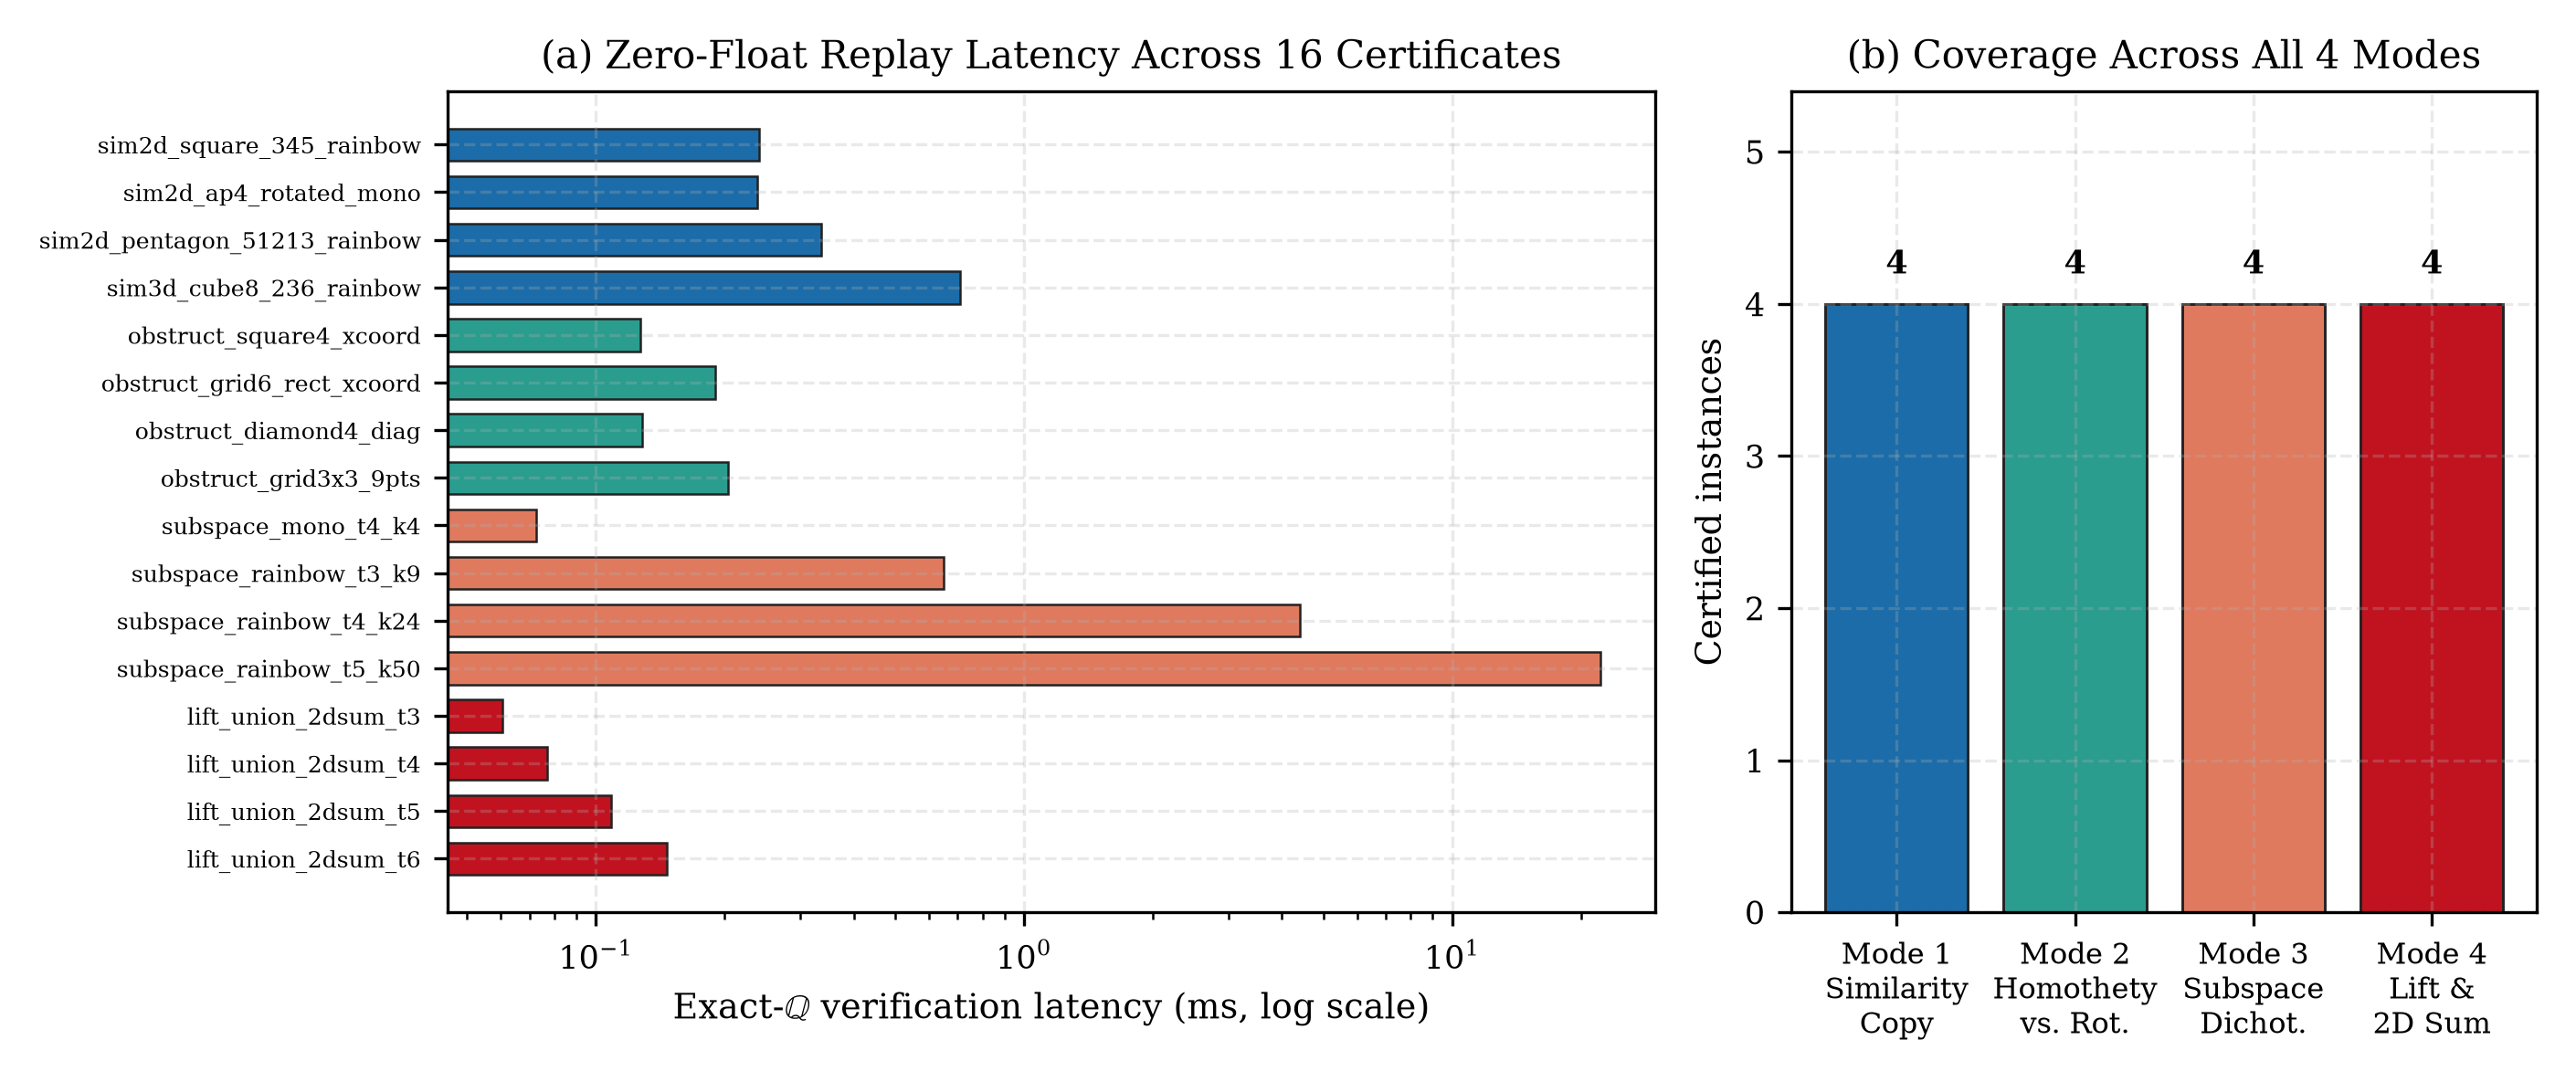
\includegraphics[width=\columnwidth]{figures/fig3_atlas_summary.png}
\caption{(a)~Zero-float replay latency across all 16 canonical \texttt{CANONICAL-GALLAI-CERT-1.0} certificates ($0.060$--$22.18\,\mathrm{ms}$, log scale). (b)~Balanced 4-per-mode coverage across all four verification modes.}
\label{fig:atlas}
\end{figure}

\begin{table}[t]
\centering
\caption{Summary of all 16 exact-$\QQ$ \texttt{CANONICAL-GALLAI-CERT-1.0} certificates (zero floating-point arithmetic; reference-machine replay latency in ms).}
\label{tab:atlas}
\resizebox{\columnwidth}{!}{%
\begin{tabular}{@{}lllr@{}}
\toprule
Certificate File (stem) & Mode & Key Exact Witness & ms \\
\midrule
\texttt{sim2d\_square\_345\_rainbow} & M1 & $d=2, t=4, s^2=1$ (rainbow) & 0.240 \\
\texttt{sim2d\_ap4\_rotated\_mono} & M1 & $d=2, t=4, s^2=4$ (mono) & 0.238 \\
\texttt{sim2d\_pentagon\_51213\_rainbow} & M1 & $d=2, t=5, s^2=1$ (rainbow) & 0.335 \\
\texttt{sim3d\_cube8\_236\_rainbow} & M1 & $d=3, t=8, s^2=1$ (rainbow) & 0.708 \\
\texttt{obstruct\_square4\_xcoord} & M2 & $t=4$: homothety $2 \to$ rot $4$ & 0.127 \\
\texttt{obstruct\_grid6\_rect\_xcoord} & M2 & $t=6$: homothety $3 \to$ rot $6$ & 0.190 \\
\texttt{obstruct\_diamond4\_diag} & M2 & $t=4$: homothety $2 \to$ rot $4$ & 0.128 \\
\texttt{obstruct\_grid3x3\_9pts} & M2 & $t=9$: homothety $3 \to$ rot $9$ & 0.203 \\
\texttt{subspace\_mono\_t4\_k4} & M3 & $t=4, k=4$, mono ($\Pr=1$) & 0.072 \\
\texttt{subspace\_rainbow\_t3\_k9} & M3 & $t=3, k=9$, rainbow ($\ge 1/4$) & 0.650 \\
\texttt{subspace\_rainbow\_t4\_k24} & M3 & $t=4, k=24$, rainbow ($\ge 1/7$) & 4.404 \\
\texttt{subspace\_rainbow\_t5\_k50} & M3 & $t=5, k=50$, rainbow ($\ge 1/11$) & 22.181 \\
\texttt{lift\_union\_2dsum\_t3} & M4 & $k=21, m=12,\; s^2=932/25$ & 0.060 \\
\texttt{lift\_union\_2dsum\_t4} & M4 & $k=124, m=42,\; s^2=449$ & 0.077 \\
\texttt{lift\_union\_2dsum\_t5} & M4 & $k=455, m=110,\; s^2=75217/25$ & 0.108 \\
\texttt{lift\_union\_2dsum\_t6} & M4 & $k=1266, m=240,\; s^2=14504$ & 0.147 \\
\bottomrule
\end{tabular}}
\end{table}

\section{Scope, Limitations, and Conclusion}\label{sec:conclusion}
This work machine-checks the finite algebraic, similarity-geometric, subspace-equivalence, and union-bound structure of Randall Shaw's canonical Euclidean Gallai theorem~\cite{randallshaw2026gallai}, and delivers a zero-float exact-$\QQ$ certificate auditor across 2D/3D similarity copies, homothety obstructions, $\ker(H)$ rainbow witnesses, and lift/similarity-sum identities. It does \emph{not} formalize the Ramsey-theoretic DGPV partition theorem~\cite{deuber1983canonical} or irrational real configurations $S \subset \mathbb{R}^d$ in Lean~4. Within its verified scope, the combined Lean~4 kernel and \texttt{CANONICAL-GALLAI-CERT-1.0} auditor provide exact, manifest-locked verification for canonical Euclidean Gallai witnesses.

\bibliographystyle{plain}
\bibliography{references}
\end{document}
